%---------------------------------------------------------------------
%                          Cap\'itulo 4
%---------------------------------------------------------------------
\chapter{Aspectos operativos}
\section{Cronograma}
El cronograma planteado se puede ver en la figura \ref{fig:cronograma}

\begin{figure}[h]
    \centering
    \captionsetup{justification=centering}
    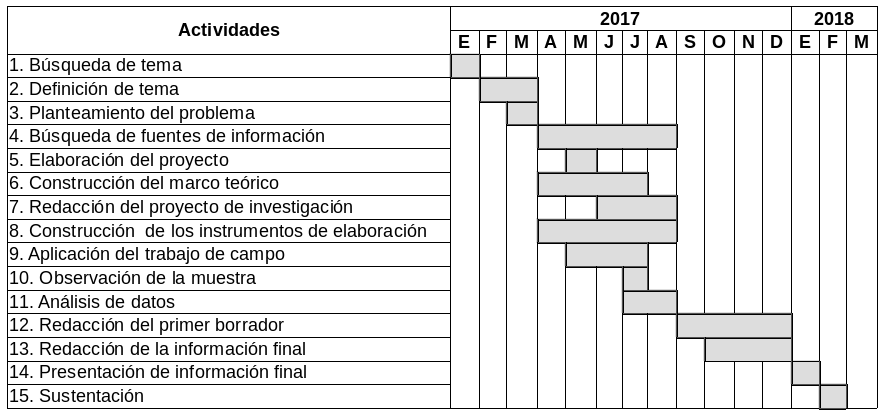
\includegraphics[width=1.0\textwidth]{Imagenes/Bitmap/cronograma}
    \caption{Cronograma de trabajo}
    \label{fig:cronograma}
\end{figure}

\section{Presupuesto y financiamiento}
El presupuesto se puede ver en la tabla \ref{t:presupuesto}.

El financiamiento sera por

\begin{table}[]
  \centering
  \caption{Presupuesto}
  \label{t:presupuesto}
  \begin{tabular}{|l|l|l|l|}
    \hline
    Detalle & Prec. Unit. & Cantidad & Sub Total \\ \hline
    &  &  &  \\ \hline
    &  &  &  \\ \hline
  \end{tabular}
\end{table}

\section{Matriz de consistencia}
%\section{Matriz de instrumentos}
%\section{Referencias bibliograficas}
\section{Instrumentos de recolecci\'on de datos}
